\documentclass[twoside]{book}

% Packages required by doxygen
\usepackage{fixltx2e}
\usepackage{calc}
\usepackage{doxygen}
\usepackage[export]{adjustbox} % also loads graphicx
\usepackage{graphicx}
\usepackage[utf8]{inputenc}
\usepackage{makeidx}
\usepackage{multicol}
\usepackage{multirow}
\PassOptionsToPackage{warn}{textcomp}
\usepackage{textcomp}
\usepackage[nointegrals]{wasysym}
\usepackage[table]{xcolor}

% Font selection
\usepackage[T1]{fontenc}
\usepackage[scaled=.90]{helvet}
\usepackage{courier}
\usepackage{amssymb}
\usepackage{sectsty}
\renewcommand{\familydefault}{\sfdefault}
\allsectionsfont{%
  \fontseries{bc}\selectfont%
  \color{darkgray}%
}
\renewcommand{\DoxyLabelFont}{%
  \fontseries{bc}\selectfont%
  \color{darkgray}%
}
\newcommand{\+}{\discretionary{\mbox{\scriptsize$\hookleftarrow$}}{}{}}

% Page & text layout
\usepackage{geometry}
\geometry{%
  a4paper,%
  top=2.5cm,%
  bottom=2.5cm,%
  left=2.5cm,%
  right=2.5cm%
}
\tolerance=750
\hfuzz=15pt
\hbadness=750
\setlength{\emergencystretch}{15pt}
\setlength{\parindent}{0cm}
\setlength{\parskip}{3ex plus 2ex minus 2ex}
\makeatletter
\renewcommand{\paragraph}{%
  \@startsection{paragraph}{4}{0ex}{-1.0ex}{1.0ex}{%
    \normalfont\normalsize\bfseries\SS@parafont%
  }%
}
\renewcommand{\subparagraph}{%
  \@startsection{subparagraph}{5}{0ex}{-1.0ex}{1.0ex}{%
    \normalfont\normalsize\bfseries\SS@subparafont%
  }%
}
\makeatother

% Headers & footers
\usepackage{fancyhdr}
\pagestyle{fancyplain}
\fancyhead[LE]{\fancyplain{}{\bfseries\thepage}}
\fancyhead[CE]{\fancyplain{}{}}
\fancyhead[RE]{\fancyplain{}{\bfseries\leftmark}}
\fancyhead[LO]{\fancyplain{}{\bfseries\rightmark}}
\fancyhead[CO]{\fancyplain{}{}}
\fancyhead[RO]{\fancyplain{}{\bfseries\thepage}}
\fancyfoot[LE]{\fancyplain{}{}}
\fancyfoot[CE]{\fancyplain{}{}}
\fancyfoot[RE]{\fancyplain{}{\bfseries\scriptsize Generated by Doxygen }}
\fancyfoot[LO]{\fancyplain{}{\bfseries\scriptsize Generated by Doxygen }}
\fancyfoot[CO]{\fancyplain{}{}}
\fancyfoot[RO]{\fancyplain{}{}}
\renewcommand{\footrulewidth}{0.4pt}
\renewcommand{\chaptermark}[1]{%
  \markboth{#1}{}%
}
\renewcommand{\sectionmark}[1]{%
  \markright{\thesection\ #1}%
}

% Indices & bibliography
\usepackage{natbib}
\usepackage[titles]{tocloft}
\setcounter{tocdepth}{3}
\setcounter{secnumdepth}{5}
\makeindex

% Hyperlinks (required, but should be loaded last)
\usepackage{ifpdf}
\ifpdf
  \usepackage[pdftex,pagebackref=true]{hyperref}
\else
  \usepackage[ps2pdf,pagebackref=true]{hyperref}
\fi
\hypersetup{%
  colorlinks=true,%
  linkcolor=blue,%
  citecolor=blue,%
  unicode%
}

% Custom commands
\newcommand{\clearemptydoublepage}{%
  \newpage{\pagestyle{empty}\cleardoublepage}%
}

\usepackage{caption}
\captionsetup{labelsep=space,justification=centering,font={bf},singlelinecheck=off,skip=4pt,position=top}

%===== C O N T E N T S =====

\begin{document}

% Titlepage & ToC
\hypersetup{pageanchor=false,
             bookmarksnumbered=true,
             pdfencoding=unicode
            }
\pagenumbering{roman}
\begin{titlepage}
\vspace*{7cm}
\begin{center}%
{\Large My Project }\\
\vspace*{1cm}
{\large Generated by Doxygen 1.8.11}\\
\end{center}
\end{titlepage}
\clearemptydoublepage
\tableofcontents
\clearemptydoublepage
\pagenumbering{arabic}
\hypersetup{pageanchor=true}

%--- Begin generated contents ---
\chapter{File Index}
\section{File List}
Here is a list of all files with brief descriptions\+:\begin{DoxyCompactList}
\item\contentsline{section}{\hyperlink{Lab1_8c}{Lab1.\+c} }{\pageref{Lab1_8c}}{}
\end{DoxyCompactList}

\chapter{File Documentation}
\hypertarget{InsertSorter_8cpp}{}\section{Insert\+Sorter.\+cpp File Reference}
\label{InsertSorter_8cpp}\index{Insert\+Sorter.\+cpp@{Insert\+Sorter.\+cpp}}
{\ttfamily \#include $<$iostream$>$}\\*
Include dependency graph for Insert\+Sorter.\+cpp\+:
\nopagebreak
\begin{figure}[H]
\begin{center}
\leavevmode
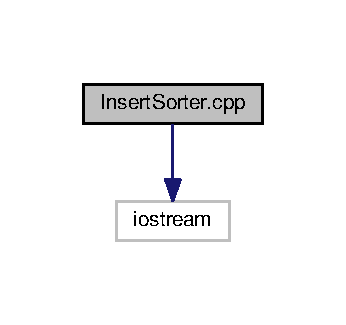
\includegraphics[width=166pt]{InsertSorter_8cpp__incl}
\end{center}
\end{figure}
\subsection*{Functions}
\begin{DoxyCompactItemize}
\item 
void \hyperlink{InsertSorter_8cpp_a77e75ec40f30cb929a156c95021ba1d7}{sort} (int arr\mbox{[}$\,$\mbox{]}, int length)
\item 
void \hyperlink{InsertSorter_8cpp_a18fb5f6ca8c8d4e2b5491c9400e30612}{move\+Down} (int arr\mbox{[}$\,$\mbox{]}, int n, int replace)
\item 
void \hyperlink{InsertSorter_8cpp_a08dc77614f804c97506e4ecd6c167647}{display} (int arr\mbox{[}$\,$\mbox{]}, int length)
\item 
int \hyperlink{InsertSorter_8cpp_ae66f6b31b5ad750f1fe042a706a4e3d4}{main} ()
\end{DoxyCompactItemize}


\subsection{Function Documentation}
\index{Insert\+Sorter.\+cpp@{Insert\+Sorter.\+cpp}!display@{display}}
\index{display@{display}!Insert\+Sorter.\+cpp@{Insert\+Sorter.\+cpp}}
\subsubsection[{\texorpdfstring{display(int arr[], int length)}{display(int arr[], int length)}}]{\setlength{\rightskip}{0pt plus 5cm}void display (
\begin{DoxyParamCaption}
\item[{int}]{arr\mbox{[}$\,$\mbox{]}, }
\item[{int}]{length}
\end{DoxyParamCaption}
)}\hypertarget{InsertSorter_8cpp_a08dc77614f804c97506e4ecd6c167647}{}\label{InsertSorter_8cpp_a08dc77614f804c97506e4ecd6c167647}

\begin{DoxyCode}
55 \{
56    cout << endl;
57    \textcolor{keywordflow}{for}(\textcolor{keywordtype}{int} k=0; k<length; k++)
58       cout << arr[k] << \textcolor{stringliteral}{" "};
59    cout << endl;
60 \}\end{DoxyCode}
\index{Insert\+Sorter.\+cpp@{Insert\+Sorter.\+cpp}!main@{main}}
\index{main@{main}!Insert\+Sorter.\+cpp@{Insert\+Sorter.\+cpp}}
\subsubsection[{\texorpdfstring{main()}{main()}}]{\setlength{\rightskip}{0pt plus 5cm}int main (
\begin{DoxyParamCaption}
{}
\end{DoxyParamCaption}
)}\hypertarget{InsertSorter_8cpp_ae66f6b31b5ad750f1fe042a706a4e3d4}{}\label{InsertSorter_8cpp_ae66f6b31b5ad750f1fe042a706a4e3d4}

\begin{DoxyCode}
16 \{
17    \textcolor{keywordtype}{int} a1[5] = \{9, 23, 1, 77, 43\};
18    \textcolor{keywordtype}{int} a2[10] = \{28, 7, 14, 73, 2, 52, 100, 32, 10, -5\};
19    \textcolor{keywordtype}{int} a3[7] = \{67, 18, 25, 0, 704, 37, 8\};
20 
21    cout << \textcolor{stringliteral}{"\(\backslash\)nOriginal arrays: "} << endl;
22    \hyperlink{InsertSorter_8cpp_a08dc77614f804c97506e4ecd6c167647}{display}(a1, 5);
23    \hyperlink{InsertSorter_8cpp_a08dc77614f804c97506e4ecd6c167647}{display}(a2, 10);
24    \hyperlink{InsertSorter_8cpp_a08dc77614f804c97506e4ecd6c167647}{display}(a3, 7);
25 
26    \hyperlink{InsertSorter_8cpp_a77e75ec40f30cb929a156c95021ba1d7}{sort}(a1, 5);
27    \hyperlink{InsertSorter_8cpp_a77e75ec40f30cb929a156c95021ba1d7}{sort}(a2, 10);
28    \hyperlink{InsertSorter_8cpp_a77e75ec40f30cb929a156c95021ba1d7}{sort}(a3, 7);
29 
30    cout << \textcolor{stringliteral}{"\(\backslash\)nSorted arrays: "} << endl;
31    \hyperlink{InsertSorter_8cpp_a08dc77614f804c97506e4ecd6c167647}{display}(a1, 5);
32    \hyperlink{InsertSorter_8cpp_a08dc77614f804c97506e4ecd6c167647}{display}(a2, 10);
33    \hyperlink{InsertSorter_8cpp_a08dc77614f804c97506e4ecd6c167647}{display}(a3, 7);
34 
35    \textcolor{keywordflow}{return} 0;
36 \}
\end{DoxyCode}


Here is the call graph for this function\+:
\nopagebreak
\begin{figure}[H]
\begin{center}
\leavevmode
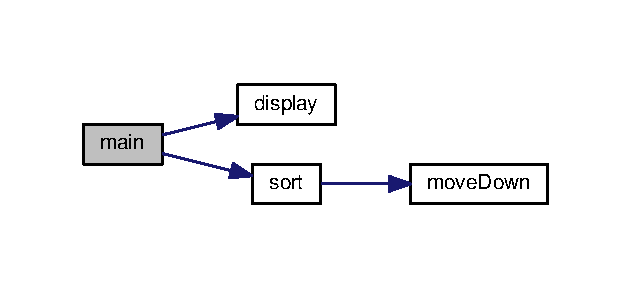
\includegraphics[width=303pt]{InsertSorter_8cpp_ae66f6b31b5ad750f1fe042a706a4e3d4_cgraph}
\end{center}
\end{figure}


\index{Insert\+Sorter.\+cpp@{Insert\+Sorter.\+cpp}!move\+Down@{move\+Down}}
\index{move\+Down@{move\+Down}!Insert\+Sorter.\+cpp@{Insert\+Sorter.\+cpp}}
\subsubsection[{\texorpdfstring{move\+Down(int arr[], int n, int replace)}{moveDown(int arr[], int n, int replace)}}]{\setlength{\rightskip}{0pt plus 5cm}void move\+Down (
\begin{DoxyParamCaption}
\item[{int}]{arr\mbox{[}$\,$\mbox{]}, }
\item[{int}]{n, }
\item[{int}]{replace}
\end{DoxyParamCaption}
)}\hypertarget{InsertSorter_8cpp_a18fb5f6ca8c8d4e2b5491c9400e30612}{}\label{InsertSorter_8cpp_a18fb5f6ca8c8d4e2b5491c9400e30612}

\begin{DoxyCode}
49 \{
50    arr[n+1] = arr[n];
51    arr[n] = replace;
52 \}
\end{DoxyCode}
\index{Insert\+Sorter.\+cpp@{Insert\+Sorter.\+cpp}!sort@{sort}}
\index{sort@{sort}!Insert\+Sorter.\+cpp@{Insert\+Sorter.\+cpp}}
\subsubsection[{\texorpdfstring{sort(int arr[], int length)}{sort(int arr[], int length)}}]{\setlength{\rightskip}{0pt plus 5cm}void sort (
\begin{DoxyParamCaption}
\item[{int}]{arr\mbox{[}$\,$\mbox{]}, }
\item[{int}]{length}
\end{DoxyParamCaption}
)}\hypertarget{InsertSorter_8cpp_a77e75ec40f30cb929a156c95021ba1d7}{}\label{InsertSorter_8cpp_a77e75ec40f30cb929a156c95021ba1d7}

\begin{DoxyCode}
39 \{
40    \textcolor{keywordflow}{for}(\textcolor{keywordtype}{int} k=0; k<length-1; k++)
41    \{
42       \textcolor{keywordtype}{int} curr = arr[k+1]; \textcolor{comment}{//curr is the first element of the unsorted array                               
                                                                                                       }
43       \textcolor{keywordflow}{for}(\textcolor{keywordtype}{int} j=k; j>=0 && arr[j] > curr; j--) \textcolor{comment}{//goes through sorted array from bottom to top              
                                                                                                       }
44          \hyperlink{InsertSorter_8cpp_a18fb5f6ca8c8d4e2b5491c9400e30612}{moveDown}(arr, j, curr);
45    \}
46 \}
\end{DoxyCode}


Here is the call graph for this function\+:
\nopagebreak
\begin{figure}[H]
\begin{center}
\leavevmode
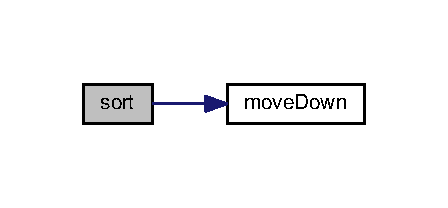
\includegraphics[width=215pt]{InsertSorter_8cpp_a77e75ec40f30cb929a156c95021ba1d7_cgraph}
\end{center}
\end{figure}



%--- End generated contents ---

% Index
\backmatter
\newpage
\phantomsection
\clearemptydoublepage
\addcontentsline{toc}{chapter}{Index}
\printindex

\end{document}
